Sequential Data is any kind of data where the order matters. Two types of sequential data are commonly studied in machine learning: \textit{sequence} and \textit{time-series}. A sequence is an ordered list of nominal values, while a time-series is an ordered list of numbers and is usually taken at successive equally spaced points in time. For instance, sequences are used to represent data such as sentences (sequences of words), while time-series are often used to represent data such as stock prices, temperature readings, and electricity consumption readings. 

When the training target is organized as a sequence, the model should not only learn the correct output combination, but also the ordering patterns. For example, in machine translation task, along with making a translation correct, the model should also find the best way to order each word in the translation. Different permutations of a sequence of words have very different meanings and readabilities in natural language. Similarly, in a motion planning system, a robot is trained to find a sequence of valid configurations that controls it to move from the source to the destination. Different orders of configurations (e.g. ``move up, move left'' and ``move left, move up'') generate different paths, and result in different interactions with the environment. In multi-label classification (studied in this chapter), different latent label orders lead different modeling outputs.

In our proposed system, the job of the base model is to generate $p(z|x)$, the probability of a latent sequence conditioned on the input. This step is usually called sequence prediction in machine learning, which uses historical sequence information to predict the next value or values in the future sequence. In addition to estimating $p(z|x)$ by using sequence prediction models, we also need to calculate the other term used in equation \ref{eq2}, i.e. $p(y|z)$. This calculation is usually modeled as a task to predict the target $y$ based on latent sequence $z$. We want $p(y|z)$ to be easily computable in this framework, and since $y$ is typically highly correlated with $z$ we will modeled it based on $z$. This is a key insight that motivates the latent variable paradigm. 


One of the most important topics in a machine learning task is the selection of the base model for comparison. Learning such models of sequences is a long-standing machine learning challenge and historically the domain of dynamic Bayesian networks (DBNs) such as hidden markov models (HMMs). The dominance of DBN-based approaches has been recently overturned by a resurgence of interest in neural network based approaches. A recurrent neural network (RNN) is able to encode the latent states into high-dimensional representations in a recurrent way, and then handle both variable-length input and output. The RNN model decomposes the joint probability over full latent sequence as a product of individual probability of each latent value in the sequence based on chain rule. Most recently, Neural Transformer \cite{vaswani2017attention}, improved from RNN, removes the dependency between adjacent RNN nodes, and allows each node to directly condition on every previous node (not just the previous one). In figure \ref{fig:model_c2}, we show the model architectures of HMM and RNN. As we can see, they both consist of two parts: (1) a transition function that determines the evolution of the internal state representation (i.e. $s_i=f(s_{i-1})$ and $h_i=f(h_{i-1})$), and (2) a mapping from the state to the output (i.e. $x_i=f(s_i)$ and $y_i=f(h_i)$). Advantages of using NN models over DBNs is that DBNs have typically been limited either to relatively simple state transition structures or to relatively simple internal state structure (e.g., the HMM state space consists of a single set of mutually exclusive states). In other words, NN based models are more powerful and capable of learning a better representations compared to DBNs. We use RNN and Transformer as our base models.

\begin{figure}[t] 
\centering
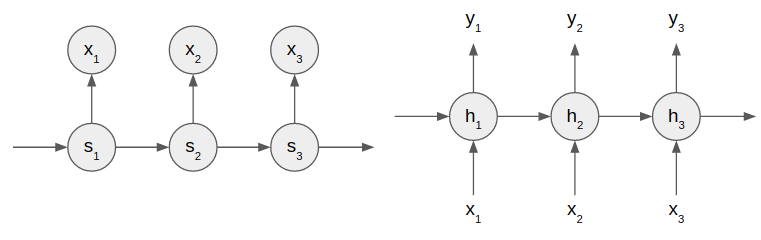
\includegraphics[width=1.0\columnwidth]{Images/rnn_hmm.png} 
  \caption{We plot the structure of HMM in the left side and RNN in the right side. For simplicity, we omit some parameters in the model. HMM is a generative model, where $x$ represents the observation and $s$ represents the hidden state. RNN is a discriminative model, where $x$ represents input features, $h$ represents hidden state representation, and $y$ represents model outputs.}
\end{figure}\label{fig:model_c2} 

Many recent work studying latent sequential data with RNN focus on adding uncertainty to the hidden states $h$ of the models. Inspired by variational autoencoder, Chung \cite{chung2015recurrent} first propose to use high-level latent random variables to model the kind of variability observed in highly structured sequential data. Following this idea, Fraccaro \cite{fraccaro2016sequential} explicitly add a stochastic layer to RNN to model uncertainty of RNN hidden states. In their setup, latent variable $z$ is just a sequence of hidden representations of input $x$, e.g. $z$ is a vector representation of input waveform in speech recognition task. On the contrary, the other line of studying latent sequential data is to explicitly translate latent sequence $z$ into interpretable variables or features. Our work fall into the later track. To solve real-world tasks, we manage to find the interpretable intermediate state to bridge the gap between input and output, and also integrate the domain knowledge and task-specific constraints together to build an end-to-end solution. Specifically, we investigate the interpretation of z and its possible values that connect input $x$ and output $y$, and propose novel approaches to make our model fit to real world tasks, such as handling inputs from multiple sources or regularizing contributions of different features.


In this chapter, we focus on discussing latent sequence in two text-based real world tasks, where sequential latent information are utilized. In section \ref{sec:2-1}, we first study a scenario that a set prediction problem being decomposed into latent sequence prediction problem in multi-label classification, and then in section \ref{sec:2-2} we discuss how a similar idea can be used to solve knowledge based question answering task (KBQA).
